\chapter{LHC-ATLAS実験}
\label{chapter2}

LHC-ATLAS 実験は、LHC (Large Hadron Collider)を用いた陽子–陽子衝突によって生成された粒子を ATLAS (A Troidal LHC ApparatuS)検出器によって検出し、標準模型の精密測定や新粒子探索などを行う実験である [5]。LHC は 2018 年に Run-2 を終了し、2019 年から 2021 年にかけて LHC 及び ATLAS 検出器のアップグレードが行われ、2022 年から Run-3 が開始された。

\section{LHC加速器}
\label{section2-1}

Large Hadron Collider (LHC)は、スイスのジュネーブ郊外にある欧州素粒子原子核研究機構 (CERN)の地下に建設された周長約 27 km の世界最大の大型ハドロン衝突型加速器である。LHC加速器の概略図を図\ref{fig:LHC加速器}に示す。
LHC加速器では高いエネルギーで陽子を衝突させることにより、TeV スケールまでの物理事象を広く調べることを目的とし様々な実験を行っている。

\begin{figure}[tb]
  \centering
  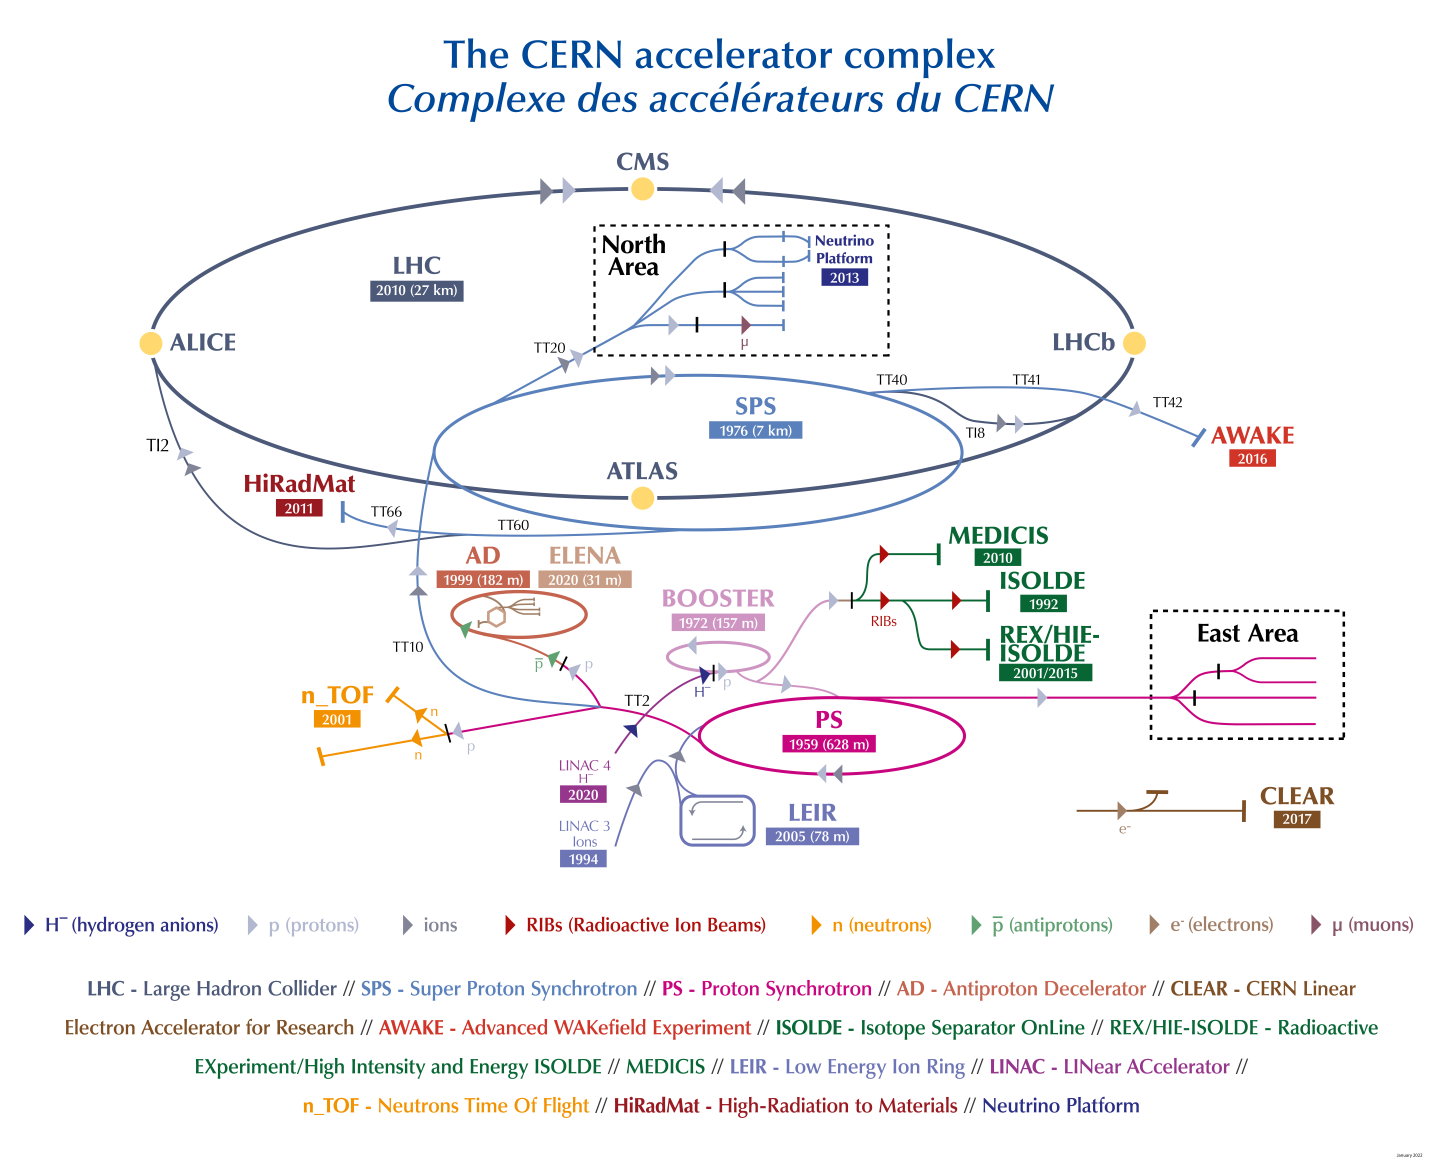
\includegraphics[clip]{fig/2/accel_complex-v2022_complex.png}
  \caption{LHC加速器の概略図}
  \label{fig:LHC加速器}
\end{figure}


LHCに陽子ビームを入射する前に、いくつかの前段加速器を使用し加速される。
初めに線源からの陽子は 線形加速器である LINAC2 で 50MeV まで加速される。第二段階は、Proton Synchrotron Booster (PSB) で1.4GeVまで加速される。Proton Synchrotron (PS) でビームを26GeVまで加速し、40MHzのバンチ構造を形成する。
その後、Super Proton Synchrotron (SPS) で450GeVまで加速された後、ビームはLHCに入射される。
LHCは陽子ビームが反対方向に周回するための2つのリングから構成されており、4か所ある衝突点にそれぞれ検出器が設置されている。
その衝突点の一つにATLAS 検出器が設置され、陽子同士の衝突から生成される粒子を検出する。
 他3箇所にも検出器が設置されており、それぞれCMS(Compact Muon Solenoid)、LHCb (Large Hadron Collider b)、ALICE (A Large Ion Collider Experiment)である。
 ATLAS と CMS の2つの検出器は、標準模型の検証から標準模型を超える現象の探索まで可能な汎用検出器である。
 LHCb と呼ばれる検出器は、B-ハドロン系の物理を研究するために設計されたものである。
 最後の ALICE は、QCD 現象を探るために重イオン衝突の研究に最適化された検出器である。

LHC

\section{ATLAS実験}
\label{section2-2}
\subsection{ATLAS検出器}
ATLAS検出器は、LHCの衝突点の1つに設置された、直径25m、長さ44mの円筒形の大型汎用検出器である。
ATLAS検出器は複数の検出器を組み合わせて構成されており、内側から内部飛跡検出器、カロリメータ、ミューオンスペクトロメータといった検出器が設置されている。また、内部飛跡検出器とカロリメータの間には超電導ソレノイド磁石、カロリメータの外側にはトロイド磁石がそれぞれ設置されており、磁場によって曲げられた荷電粒子の曲率半径から運動量の算出を行っている。

\begin{figure}[tb]
  \centering
  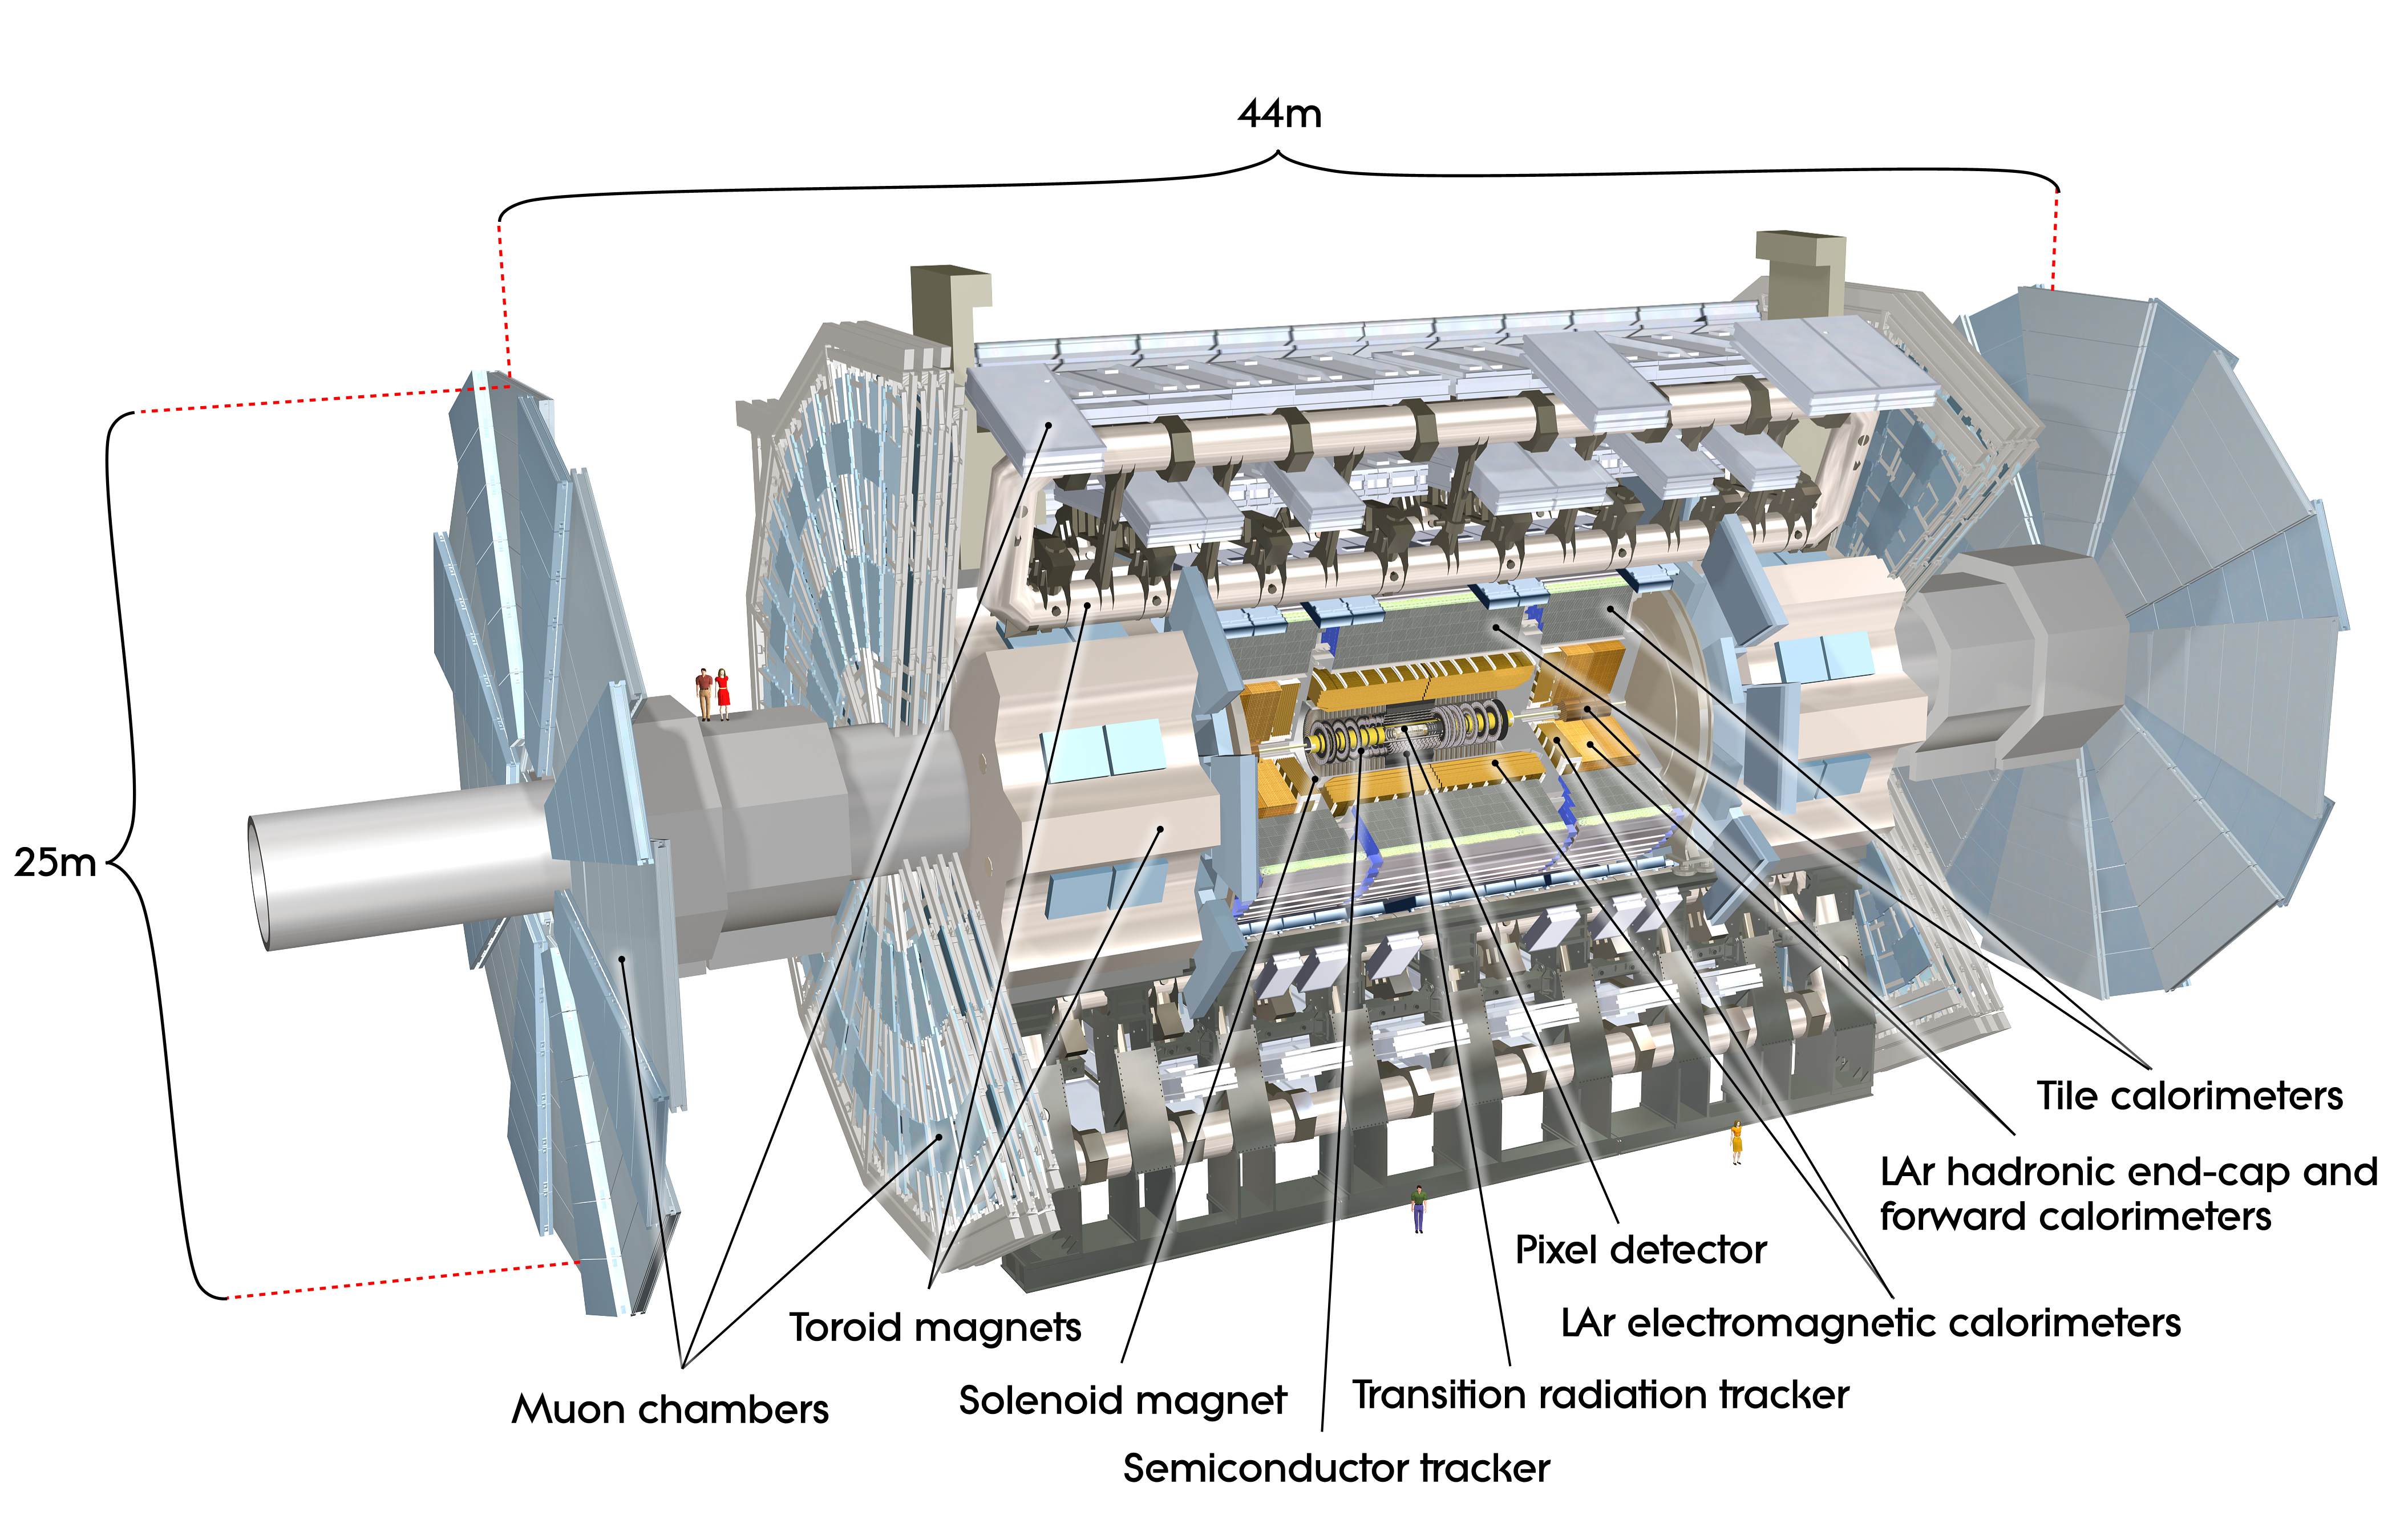
\includegraphics[clip,width=14cm]{fig/2/0803012_01.jpg}
  \caption{ATLAS検出器の全体図}
  \label{fig:ATLAS検出器}
\end{figure}


\subsection{ATLAS検出器における座標系}
ATLAS検出器における座標系を示す(図\ref{fig:a})。検出器の中心を原点とし、ビーム軸に沿ってz軸を取る。地面に対して平行方向にx軸を取り、垂直方向にy軸を取る直行座標系および、円筒座標系を設定する。また、ATLAS実験では、$\eta=-ln(tan\theta/2)$と定義される擬ラピディティ$\eta$を使用する。

\begin{figure}[tb]
  \centering
  \includegraphics[clip, width=14cm]{fig/2/atlas_coordinate_fix.pdf}
  \caption{ATLAS検出器における座標系}
  \label{fig:a}
\end{figure}

衝突点を原点とし、ビーム軸に沿ってz軸を取る。地面に水平方向にx軸を取り、x-z平面に垂直方向にy軸を取る。

\subsection{内部飛跡検出器}

\begin{figure}
    \centering
    \begin{minipage}[b]{0.3\linewidth}
        \centering
        \includegraphics[clip, width=8cm]{fig/2/inner_detectoer1.jpg}
        \vspace{10pt}
        \subcaption{内部飛跡検出器の概略図}
        \label{fig:内部飛跡検出器の概略図1}
    \end{minipage}
    \hfill
    \begin{minipage}[b]{0.5\linewidth}
        \centering
        \includegraphics[clip, width=7cm]{fig/2/inner_detector2.jpg}
        \vspace{10pt}
        \subcaption{内部飛跡検出器の概略図}
        \label{fig:内部飛跡検出器の概略図2}
    \end{minipage}
    \caption{Three simple graphs}
    \label{fig:three graphs}
\end{figure}



\subsection{カロリメータ}
カロリメータは、内部飛跡検出器の外側に設置されており、LHCでの陽子衝突で生成された粒子のエネルギー及び位置を測定する役割を担っている。
ATLAS検出器に設置されているカロリメータは、吸収層と検出層からなるサンプリングカロリメータであり、高密度物質の吸収層で粒子シャワーを起こし、検出層で電気信号に変えることで粒子の同定を行っている。
ATLASのカロリメータは、電磁カロリメータとハドロンカロリメータの2種類設置されている。

\subsubsection{・電磁カロリメータ}
電磁カロリーメーターは、$|\eta|<1.5$をカバーするバレルカロリメータと、$1.4<|\eta|<3.4$をカバーするエンドキャプカロリメータに分かれている。
バレル部とエンドキャプ部ともに、吸収層の鉛と検出層の液体アルゴンで構成されたカロリメータであり、電磁相互作用を起こす光子や電子のエネルギーと位置を測定する役割を担っている。

\subsubsection{・ハドロンカロリメータ}
ハドロンカロリメータは電磁カロリメータの外側に設置されており、タイルカロリーメータ、エンドキャップカロリーメータ、フォワードカロリーメータの3つに分類され、それぞれ異なる$|\eta=$範囲をカバーする。バレル部では、鉛と

\subsection{ミューオンスペクトロメータ}
\label{section2-2-4}
バレル領域は |η| < 1.05、エンドキャップ領域は |η| > 1.05
に対応する。また、η > 0 を A-side、η < 0 を C-side と呼ぶ。


\subsubsection{・Thin Gap Chambers (TGC)}



\subsection{マグネットシステム}
\subsubsection{・ソレノイド磁石}




